%%%%%%%%%%%%%%%%%%%%%%%%%%%%%%%%%%%%%%%%%
% Journal Article
% LaTeX Template
% Version 2.0 (February 7, 2023)
%
% This template originates from:
% https://www.LaTeXTemplates.com
%
% Author:
% Vel (vel@latextemplates.com)
%
% License:
% CC BY-NC-SA 4.0 (https://creativecommons.org/licenses/by-nc-sa/4.0/)
%
% NOTE: The bibliography needs to be compiled using the biber engine.
%
%%%%%%%%%%%%%%%%%%%%%%%%%%%%%%%%%%%%%%%%%

%----------------------------------------------------------------------------------------
%	PACKAGES AND OTHER DOCUMENT CONFIGURATIONS
%----------------------------------------------------------------------------------------

\documentclass[
	a4paper, % Paper size, use either a4paper or letterpaper
	10pt, % Default font size, can also use 11pt or 12pt, although this is not recommended
	unnumberedsections, % Comment to enable section numbering
	twoside, % Two side traditional mode where headers and footers change between odd and even pages, comment this option to make them fixed
]{LTJournalArticle}

% \addbibresource{sample.bib} % BibLaTeX bibliography file

\runninghead{} % A shortened article title to appear in the running head, leave this command empty for no running head

\setcounter{page}{1} % The page number of the first page, set this to a higher number if the article is to be part of an issue or larger work

%----------------------------------------------------------------------------------------
%	TITLE SECTION
%----------------------------------------------------------------------------------------

\title{FEATURE} % Article title, use manual lines breaks (\\) to beautify the layout

% Authors are listed in a comma-separated list with superscript numbers indicating affiliations
% \thanks{} is used for any text that should be placed in a footnote on the first page, such as the corresponding author's email, journal acceptance dates, a copyright/license notice, keywords, etc
\author{%
	Wagner Nicolas\thanks{Corresponding author: \href{mailto:nicolas@feature.sh}{nicolas@feature.sh}\\ \textbf{Published:} December 6, 2023}
}

% Full-width abstract
\renewcommand{\maketitlehookd}{%
    \begin{abstract}
        \noindent FEATURE redefines engagement in open-source development by integrating cryptocurrency rewards into development tasks on GitHub. This approach creates the necessary conditions to encourage developers to fully invest in their contributions, while ensuring quality deliverables for the issuer. FEATURE's Atomic Contract facilitates secure and transparent transactions, providing clear and direct compensation for developers. Thus, FEATURE transforms open-source collaboration into a straightforward and rewarding experience, accelerating the evolution of the Open Source development ecosystem.
    \end{abstract}
}

%----------------------------------------------------------------------------------------

\begin{document}

\maketitle % Output the title section

%----------------------------------------------------------------------------------------
%	ARTICLE CONTENTS
%----------------------------------------------------------------------------------------

\section{Introduction}

Since the advent of the Internet, work processes have undergone a radical transformation, shifting from often localized, individual, and manual methods to global, collaborative, and digitally connected approaches. Emails, discussion forums, and the earliest websites have significantly contributed to the widespread adoption of collaborative work. One of the most significant advances of these tools is the ability to communicate and share information instantly on a global scale, fostering the growth of remote and independent work.

Professionals began to exploit these new opportunities to offer their skills and services to a global audience. Concurrently, compensation models evolved significantly. Traditional salaried employment faced strong competition from hourly, project-based, and even task-based (microtasking) payment models.

This evolution of models generates, on one hand, greater competition benefiting recruiters, but on the other hand, it allows independents to access a broader and more diverse range of missions. To meet this need to connect clients and freelancers, numerous freelancing marketplaces emerged, such as Upwork or Fiverr.

These platforms adapt to the changing needs of the labor market. They can offer advanced features such as rating systems, project management tools, and work progress tracking services. The latest trends and technologies in recent years, such as artificial intelligence and blockchain, are driving some of these platforms to innovate and offer an increasingly attractive service.

FEATURE positions itself at the forefront of this transformation. By integrating blockchain smart contracts with cryptocurrency rewards directly on GitHub, FEATURE adds an economic incentive layer to a tool that developers are accustomed to working with. Rewarding development tasks in cryptocurrencies via GitHub ensures secure and transparent transactions, propelling collaborative innovation to new horizons.

%------------------------------------------------

\section{GitHub, Open-Source, and FEATURE}

GitHub initially emerged as a code hosting and version tracking solution with a web interface. Its graphical interface displays the various evolutions of the code executed by the Git software. GitHub has evolved to offer a range of tools surrounding code, such as task tracking (issue tracking), project management (GitHub Project), the DevOps part (GitHub Actions), and the ability for third-party applications to integrate into its ecosystem through "extensions" on GitHub.

FEATURE leverages this GitHub extension functionality. It is also listed on the GitHub Marketplace. The GitHub integration allows for simplified management of cryptocurrency rewards. There is no need to use a third-party application to utilize it. The creation, claim, and payment of the cryptocurrency reward are done directly on GitHub. This presents two major advantages:
\begin{itemize}
\item
  for the client, since the cryptocurrency reward is directly on GitHub, it reaches developers where they are already present, increasing the power to attract a larger number of developers.
\item
  for developers, their workflow is simplified as it takes place on a platform they are accustomed to working with.
\end{itemize}

The GitHub platform has significantly contributed to Open Source as a whole, particularly in the blockchain domain. Bitcoin and Ethereum are among many examples. Open Source, which refers to software where the code is accessible to all, attracts numerous developers, but it is often a non-profit "market." For these developers, motivations can be diverse: technical (skill improvement, bug fixing for program usage...), social (building a portfolio of contributions), and economic (reward for finding security flaws...). However, these factors often do not suffice to stimulate massive participation from external developers. This is even more true when it comes to making significant contributions, which are usually the result of a small group of developers paid by a foundation or a private entity.

So, how can we further activate external contributions?

FEATURE's hypothesis is that even if there are reasons to contribute to an Open Source project (technical, social...), it is only through systemic economic incentives directly on GitHub that we can significantly increase the number of major contributions from the developer community.

Thus, FEATURE positions itself in the freelancing market in the development domain by associating a cryptocurrency reward with every GitHub task (Issue) with the aim of activating more contributors and thereby accelerating the Open Source ecosystem.

%------------------------------------------------

\section{Atomic Contract}

The idea of making payments in cryptocurrency originated in 2008 with the publication of the "Bitcoin" whitepaper. Cryptocurrency allows for peer-to-peer transactions in a secure manner, without the need for a trusted third party. This means that users can make payments directly to each other, without relying on an intermediary to validate or verify transactions.

This concept was extended to the creation of smart contracts, allowing users or programs to interact with programs that "automatically" execute predefined actions when specific conditions are met.

These smart contracts can be particularly useful for creating escrow arrangements where provisioned funds are released only under certain conditions defined by the smart contract. These specific types of programs are called Escrow Smart Contracts.

The Atomic Contract reconciles these different concepts - cryptocurrencies, smart contracts, and escrow - to execute economic transactions under specific conditions (contract) and specific to a task (atomic).

Its relevance in the freelance domain is the ability to transition from time-based remuneration, as in salaried employment, for example, or project-based, often proposed by agencies, to task-based remuneration. Development tasks are particularly well-managed on GitHub through issues. GitHub issues allow for the description of the task with a discussion thread to follow its progress and leave remarks if necessary. FEATURE adds to these issues directly in the discussion thread a cryptocurrency reward to encourage developers to undertake the task. The remuneration associated with the task is released only if conditions are met, namely the delivery deadline and the quality of the deliverable. This is how FEATURE proposes Atomic Contracts.

Remunerating by the task allows for a departure from the somewhat vague remuneration system of project-based or time-based payment. Indeed, how can one retrospectively calculate the value each developer brought to the project when its delivery may occur several weeks or months after the initial developments? This can be very complicated, especially if there is no regular tracking of contributions.

By relying on Atomic Contracts, FEATURE ensures client-developer economic transactions, giving more confidence to the developer to invest time in completing the task and for the client to manage development costs more precisely.

%------------------------------------------------

\section{Configuration}

FEATURE offers several types of configurations to best adapt to user needs in terms of user experience and security. To best meet the user's needs, it is possible to configure:

\begin{itemize}
\item
  the amount of the transaction, whether in coin (native token of a blockchain) or in token following the ERC20 standard.
\item
  and the timeframe within which the task must be completed.
\end{itemize}

\begin{figure*}[ht]
  \centering
  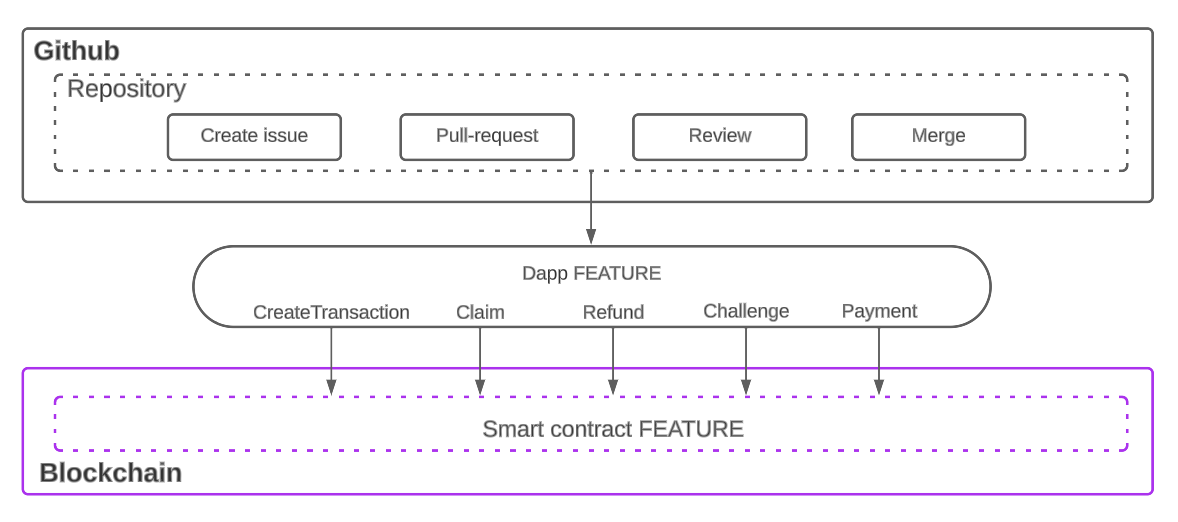
\includegraphics[width=0.88\textwidth]{media/diagram_web3_Feature.png}
  \caption{FEATURE web3 diagram - This schematic represents an overview of the workflow for the FEATURE Dapp, utilizing code management from GitHub repositories to interactions with blockchain smart contracts.}
  \label{fig:web3 diagram}
\end{figure*}

In addition to this basic configuration, it is possible to configure economic incentives to ensure the quality of the deliverable:

\begin{itemize}
\item
  the challenge period during which reviewers can challenge the developer who completed the task,
\item
  a deposit made at the time of the developer code proposal to encourage other developers to review their code,
\item
  and finally, the arbitrator to resolve the dispute between the issuer and the challenger in case of litigation, which can be a centralized arbitrator, a multisig, or a DAO (Kleros).
\end{itemize}

In addition to these configurations, it is possible to perform transactions in self-custodial or custodial mode. The advantage of custodial mode is to no longer worry about blockchain transactions. It is simply configured by provisioning a wallet and associating each GitHub label, which allows, for example, to tag issues by the difficulty of the issue, with an Atomic Contract. This mode ensures an extremely smooth experience as the Atomic Contracts will then be automatically created at the time of labeling an issue. This last mode reconciles the advantage of Atomic Contracts with a much smoother "web2 experience" for users.


%------------------------------------------------

\section{Workflow}

Let's explore the user experience by describing step by step the workflow from the creation of the Atomic Contract to its conclusion, i.e., its payment or possibly its resolution via the arbitrator:

\begin{enumerate}
\item
  creation of the GitHub issue;
\item
  labeling of the issue with a GitHub label configured with FEATURE to generate the Atomic Contract and escrow the cryptocurrency reward;
\item
  discussion about the work to be done, or in progress, directly in the discussion thread of the issue, and the refund of funds for the issuer if there were no code proposals, called pull-request, within the allotted time;
\item
  creation of a pull-request by a developer and registration of this proposal on the Atomic Contract;
\item
  code review by developers and possibly submission of a dispute if the challenger believes that the specifications have not been respected;
\item
  creation of a pull-request by a developer and registration of this proposal on the Atomic Contract;
\item
  in the event of a dispute, either the challenger will receive the developer's deposit and the Atomic Contract will be available to accept new code proposals, or the developer wins the dispute, he will then win the cryptocurrency reward and the Atomic Contract will be completed;
\item
  the merge of the pull-request to add the proposed solution implementation to the main code source.
\end{enumerate}

The diagram Figure \ref{fig:web3 diagram} summarizes these different steps.

This workflow ensures an optimal experience for both the developer, by offering an experience as close as possible to what they are accustomed to on GitHub with the assurance of being paid if they meet the specifications described in the issue, and for the issuer, who thanks to the review system can ensure a quality deliverable provided within the allotted time, which in case these requirements are not met will be refunded.

\section{Conclusion}

FEATURE offers a streamlined solution to motivate developers in contributing to Open Source projects via cryptocurrency rewards. This is actualized through the establishment of an Atomic Contract, ensuring on one hand the developer's compensation, and on the other, guaranteeing the issuer high-quality deliverables within the stipulated time frame.

This innovation aligns closely with the developer's usual workflow, both in task consultation and in code reviews, while potentially receiving cryptocurrency rewards for their efforts. For the issuer, executing offers directly on GitHub and automating them through GitHub labels not only targets developers where they are most active but also simplifies the process of offer creation.

FEATURE, thus, transforms GitHub collaboration into a more straightforward and rewarding experience, rendering it an ideal tool for accelerating code development in Open Source projects.

\end{document}
